%===============================================================================
\chapter{Virtual Reference Feedback Tunning}
\label{chapter:vfrt}
%===============================================================================
\TODO:: REVER ESTE PARAGRAFO:

Em aplica��es pr�ticas, a descri��o matematica da planta n�o � dispon�vel e o sistema deve ser identificado
baseado nas medidas obtidas deste sistema. Este assunto tem atraido a aten��o de diversos engenheiros de
controle desde 1940 com o pioneiro trabalho de Ziegler e Nichols (1942) com ajuste de controladores PID
industriais. Depois do trabalho de Ziegler e Nichols divesos trabalhos surgiram, muitos em formas de
aperfei�oamento e extens�es das tecnicas ja apresentadas, e algumas com desenvolvimentos em novas dire��es
(\cite{mcmillan1983tuning}, \cite{Haalman1965}). A caracteristica principal destes metodos � que eles podem
ser facilmente utilizados: simples experimentos sobre a planta s�o executados e simples regras 
s�o aplicadas sobre os dados obtidos. O metodo VRFT que ser� abordado aqui tem algumas destas 
caracteristicas, pois s� requer que apenas um experimento seja executado sobre a planta. 
\cite{campi_leccini_savaresi2002}

%===============================================================================
%===============================================================================
\section{Controle baseado em dados}
\label{sec:vrft_control_data_based}
%===============================================================================

O projeto de controladores baseados em dados consiste obter ou ajustar os par�metros de um modelo
para os controladores, baseado nos dados obtidos da planta em an�lise. Os dados utilizados para esta
tarefa s�o basicamente o sinal de entrada e sa�da do sistema.

Como j� foi discutido na se��o (\ref{sec:si_project_experiments}) estes dados podem ser obtidos de
diversas formas. Algumas vezes estas informa��es podem ser a opera��o normal da planta em malha
fechada com a presen�a de algum controlador, situa��o esta que tem um apelo grande em plantas
industriais, onde a parada do processo para levantamento de informa��es � indesej�vel, e muitas
vezes at� invi�vel. Se existe a possibilidade de parar a planta e aplicar-se sinais predeterminados,
o projeto de experimentos pode trazer muitas vantagens.

Seja a esperan�a de um valor $E\left [ \cdot \right ]$ definido por: \cite{ljung}

\begin{equation}
\bar{E}\left [ f(t) \right ]\equiv \lim_{N \to \infty } \frac{1}{N}\sum_{t=1}^{N}E\left [ f(t)
\right]
\label{eq:vrft_db_hope}
\end{equation}

Um sinal � dito quasi-estacionario se a m�dia e autocorrela��o do mesmo convergem para um valor
finito quando o tamanho da amostra cresce, conforme defini��o a seguir: \cite{campestrini}


\begin{defn}
\cite{ljung}

Um Sinal $s(t)$ � um processo quasi-estacionario se:
\begin{itemize}
	\item $\bar{E}\left [ s(t) \right ] = \mid m_s \mid \le C, \;\forall t$;
	\item $\bar{E}\left [ s(t)s(r) \right ] = \mid R_s(t,s) \mid \le C, \;\forall t,r$;
	\item $\lim_{N \to \infty}\frac{1}{N}\sum_{t=1}^{N}R_s(t, t-\tau)=R_s(\tau), \; \forall \tau$,
\end{itemize}
Onde $m_s(t)$ � o valor m�dio do sinal $s(t)$ e $R_s(t,r)$ � a covari�ncia do sinal $s$ nos
instantes $t$ e $r$.
\end{defn}

O ruido � um processo quasi-estacionario, que pode ser descrito como $\nu(t)=H_0(z)e(t)$, onde
$e(t)$ � ruido branco com vari�ncia $\sigma_e^2$. Ambas fun��es de transfer�ncia, $G(z)$ e $H(z)$,
s�o racionais e causais. Assume-se que $H(\infty)=1$, ou seja, a resposta impulsiva do filtro
$H_0(z)$ satisfaz $h(0)=1$. \cite{campestrini}

Na Figura (\ref{fig:vrft_db_control_loop}) � apresentado uma malha de controle onde o controlador
$C(z, \rho) \in \mathcal{C}$ onde $ \mathcal{C}$ � a classe de controladores definida pelo usu�rio.

\begin{figure}[htbp]
\center
\scalebox{1} % Change this value to rescale the drawing.
{
\begin{pspicture}(0,-1.1092187)(9.868125,1.1292187)
\pscircle[linewidth=0.04,dimen=outer](1.4,-0.08921875){0.2}
\psframe[linewidth=0.04,dimen=outer](4.4,0.31078124)(2.6,-0.48921874)
\psframe[linewidth=0.04,dimen=outer](7.2,0.31078124)(5.6,-0.48921874)
\pscircle[linewidth=0.04,dimen=outer](8.4,-0.08921875){0.2}
\psline[linewidth=0.04cm,arrowsize=0.05291667cm 2.0,arrowlength=1.4,arrowinset=0.4]{->}(0.0,-0.08921875)(1.2,-0.08921875)
\psline[linewidth=0.04cm,arrowsize=0.05291667cm 2.0,arrowlength=1.4,arrowinset=0.4]{->}(1.6,-0.08921875)(2.6,-0.08921875)
\psline[linewidth=0.04cm,arrowsize=0.05291667cm 2.0,arrowlength=1.4,arrowinset=0.4]{->}(4.4,-0.08921875)(5.6,-0.08921875)
\psline[linewidth=0.04cm,arrowsize=0.05291667cm 2.0,arrowlength=1.4,arrowinset=0.4]{->}(7.2,-0.08921875)(8.2,-0.08921875)
\psline[linewidth=0.04cm,arrowsize=0.05291667cm 2.0,arrowlength=1.4,arrowinset=0.4]{->}(8.4,0.7107813)(8.4,0.11078125)
\psline[linewidth=0.04cm,arrowsize=0.05291667cm 2.0,arrowlength=1.4,arrowinset=0.4]{->}(8.6,-0.08921875)(9.8,-0.08921875)
\psline[linewidth=0.04cm,arrowsize=0.05291667cm 2.0,arrowlength=1.4,arrowinset=0.4]{<-}(1.4,-0.28921875)(1.4,-1.0892187)
\psline[linewidth=0.04cm](1.4,-1.0892187)(9.2,-1.0892187)
\psline[linewidth=0.04cm](9.2,-1.0892187)(9.2,-0.08921875)
\usefont{T1}{ptm}{m}{n}
\rput(1.1126562,0.22078125){+}
\usefont{T1}{ptm}{m}{n}
\rput(8.112657,0.22078125){+}
\usefont{T1}{ptm}{m}{n}
\rput(8.112657,-0.37921876){+}
\usefont{T1}{ptm}{m}{n}
\rput(1.6473438,-0.37921876){-}
\usefont{T1}{ptm}{m}{n}
\rput(0.47,0.21078125){\small $r(t)$}
\usefont{T1}{ptm}{m}{n}
\rput(3.59,-0.08921875){\small $C(z, \rho)$}
\usefont{T1}{ptm}{m}{n}
\rput(6.36,-0.10921875){\small $G_0(z)$}
\usefont{T1}{ptm}{m}{n}
\rput(5.11,0.21078125){\small $u(t)$}
\usefont{T1}{ptm}{m}{n}
\rput(2.21,0.21078125){\small $\xi(t)$}
\usefont{T1}{ptm}{m}{n}
\rput(8.48,0.93078125){\small $\nu(t)$}
\usefont{T1}{ptm}{m}{n}
\rput(9.3,0.21078125){\small $y(t)$}
\end{pspicture} 
}
\caption{Rede neural recorrentes.}
\label{fig:vrft_db_control_loop}
\end{figure}

A equa��o \eqref{eq:vrft_db_closed_loop} descreve o comportamento do sistema da Figura
(\ref{fig:vrft_db_control_loop}).

\begin{equation}
T(z, \rho)=\frac{C(z,\rho)G_0(z)}{1+C(z,\rho)G_0(z)}
\label{eq:vrft_db_closed_loop}
\end{equation}

Controle baseado em dados pode ser dividido em dois grupos principais: m�todos iterativos onde
experimentos s�o realizados sobre o sistema atualizando-se o controlador, o processo ent�o � repetido
at� que se atinja um valor minimo para a fun��o custo deste sistema. O segundo grupo � o de m�todos
n�o iterativos, onde apenas com um experimento, ou um conjunto de dados, os par�metros do
controlador s�o estimados.



%===============================================================================
\section{Iterative feedback tuning}
\label{sec:vrft_control_ift}
%===============================================================================

O m�todo IFT utiliza um algoritmo iterativo para minimizar uma fun��o custo $H_2$. O m�todo
considera que o sistema � controlado por um controlador com dois graus de liberdade:

\begin{equation}
u(t)=C_r(z)r(t)-C_y(z)y(t)
\label{eq:vrft_db_ift_controller}
\end{equation}

Na Figura (\ref{fig:vrft_db_ift}) � apresentado a organiza��o dos blocos dos controladores
apresentados em \eqref{eq:vrft_db_ift_controller}, $C_r(z)$ e $C_y(z)$. O controlador pode ser
entendido como o conjunto destes dois:\cite{ift_theory_and_applications}

\begin{equation}
C(z) \equiv  \left \{ C_r(z),\, C_y(z)  \right \} 
\nonumber
\end{equation}

\begin{figure}[htbp]
\center
\scalebox{1} % Change this value to rescale the drawing.
{
\begin{pspicture}(0,-1.68)(9.48,1.72)
\usefont{T1}{ptm}{m}{n}
\rput(7.691875,1.5215625){\small $\nu(t)$}
\pscircle[linewidth=0.04,dimen=outer](4.0,0.32){0.2}
\pscircle[linewidth=0.04,dimen=outer](8.0,0.32){0.2}
\psframe[linewidth=0.04,dimen=outer](6.8,0.72)(5.2,-0.08)
\psframe[linewidth=0.04,dimen=outer](2.8,0.72)(1.2,-0.08)
\psframe[linewidth=0.04,dimen=outer](6.8,-0.88)(5.2,-1.68)
\psline[linewidth=0.04cm,arrowsize=0.05291667cm 2.0,arrowlength=1.4,arrowinset=0.4]{->}(0.0,0.32)(1.2,0.32)
\psline[linewidth=0.04cm,arrowsize=0.05291667cm 2.0,arrowlength=1.4,arrowinset=0.4]{->}(2.8,0.32)(3.8,0.32)
\psline[linewidth=0.04cm,arrowsize=0.05291667cm 2.0,arrowlength=1.4,arrowinset=0.4]{->}(4.2,0.32)(5.2,0.32)
\psline[linewidth=0.04cm,arrowsize=0.05291667cm 2.0,arrowlength=1.4,arrowinset=0.4]{->}(6.8,0.32)(7.8,0.32)
\psline[linewidth=0.04cm,arrowsize=0.05291667cm 2.0,arrowlength=1.4,arrowinset=0.4]{->}(8.2,0.32)(9.2,0.32)
\psline[linewidth=0.04cm,arrowsize=0.05291667cm 2.0,arrowlength=1.4,arrowinset=0.4]{<-}(6.8,-1.28)(8.0,-1.28)
\psline[linewidth=0.04cm](8.0,-1.28)(8.0,0.12)
\psline[linewidth=0.04cm,arrowsize=0.05291667cm 2.0,arrowlength=1.4,arrowinset=0.4]{<-}(4.0,0.12)(4.0,-1.28)
\psline[linewidth=0.04cm](4.0,-1.28)(5.2,-1.28)
\usefont{T1}{ptm}{m}{n}
\rput(8.911875,0.5215625){\small $y(t)$}
\usefont{T1}{ptm}{m}{n}
\rput(0.481875,0.5215625){\small $r(t)$}
\usefont{T1}{ptm}{m}{n}
\rput(1.901875,0.3215625){\small $C_r(z)$}
\usefont{T1}{ptm}{m}{n}
\rput(5.951875,0.3215625){\small $G_0(z)$}
\usefont{T1}{ptm}{m}{n}
\rput(5.931875,-1.2784375){\small $C_y(z)$}
\usefont{T1}{ptm}{m}{n}
\rput(4.721875,0.7215625){\small $u(t)$}
\psline[linewidth=0.04cm,arrowsize=0.05291667cm 2.0,arrowlength=1.4,arrowinset=0.4]{->}(8.0,1.32)(8.0,0.52)
\usefont{T1}{ptm}{m}{n}
\rput(4.2592187,0.1315625){-}
\end{pspicture} 
}
\caption{Diagrama de bloco do sistema utilizado na identifica��o IFT.}
\label{fig:vrft_db_ift}
\end{figure}

\begin{equation}
J(\rho)=\frac{1}{2N}E\left [ \sum_{t=1}^{N}(L_y \tilde{y}_t(\rho))^2 +\lambda  \sum_{t=1}^{N}(L_u
u_t(\rho))^2 \right ]
\label{eq:vrft_db_ift_j_cost}
\end{equation}








\begin{figure}[htbp]
\center
\scalebox{1} % Change this value to rescale the drawing.
{
\begin{pspicture}(0,-1.4292188)(9.02,1.4692187)
\pscircle[linewidth=0.04,linestyle=dashed,dash=0.16cm 0.16cm,dimen=outer](1.4,0.97078127){0.2}
\psframe[linewidth=0.04,linestyle=dashed,dash=0.16cm 0.16cm,dimen=outer](4.8,1.3707813)(3.0,0.57078123)
\psframe[linewidth=0.04,dimen=outer](7.6,1.3707813)(6.0,0.57078123)
\psline[linewidth=0.04cm,arrowsize=0.05291667cm 2.0,arrowlength=1.4,arrowinset=0.4]{->}(0.0,0.97078127)(1.2,0.97078127)
\psline[linewidth=0.04cm,linestyle=dashed,dash=0.16cm 0.16cm,arrowsize=0.05291667cm 2.0,arrowlength=1.4,arrowinset=0.4]{->}(1.6,0.97078127)(3.0,0.97078127)
\psline[linewidth=0.04cm,arrowsize=0.05291667cm 2.0,arrowlength=1.4,arrowinset=0.4]{->}(4.8,0.97078127)(6.0,0.97078127)
\psline[linewidth=0.04cm](7.6,0.97078127)(9.0,0.97078127)
\psline[linewidth=0.04cm,linestyle=dashed,dash=0.16cm 0.16cm,arrowsize=0.05291667cm 2.0,arrowlength=1.4,arrowinset=0.4]{<-}(1.4,0.7707813)(1.4,-0.02921875)
\psline[linewidth=0.04cm,linestyle=dashed,dash=0.16cm 0.16cm](1.4,-0.02921875)(8.4,-0.02921875)
\psline[linewidth=0.04cm,linestyle=dashed,dash=0.16cm 0.16cm](8.4,-0.02921875)(8.4,0.97078127)
\usefont{T1}{ptm}{m}{n}
\rput(1.1126562,1.2807813){+}
\usefont{T1}{ptm}{m}{n}
\rput(1.6473438,0.68078125){-}
\usefont{T1}{ptm}{m}{n}
\rput(0.47,1.2707813){\small $r(t)$}
\usefont{T1}{ptm}{m}{n}
\rput(3.99,0.97078127){\small $C(z, \rho)$}
\usefont{T1}{ptm}{m}{n}
\rput(6.76,0.9507812){\small $G_0(z)$}
\usefont{T1}{ptm}{m}{n}
\rput(5.51,1.2707813){\small $u(t)$}
\usefont{T1}{ptm}{m}{n}
\rput(2.25,1.2707813){\small $\bar{e}(t)$}
\usefont{T1}{ptm}{m}{n}
\rput(8.3,1.2707813){\small $y(t)$}
\psframe[linewidth=0.04,dimen=outer](6.0,-0.62921876)(3.8,-1.4292188)
\usefont{T1}{ptm}{m}{n}
\rput(4.91,-1.0492188){\small $M^{-1}(z)$}
\psline[linewidth=0.04cm](9.0,0.97078127)(9.0,-1.0292188)
\psline[linewidth=0.04cm](9.0,-1.0292188)(6.0,-1.0292188)
\psline[linewidth=0.04cm](3.8,-1.0292188)(0.0,-1.0292188)
\psline[linewidth=0.04cm](0.0,-1.0292188)(0.0,0.97078127)
\end{pspicture} 
}
\caption{Rede neural recorrentes.}
\label{fig:nl_models_neural_recurrent}
\end{figure}

% ===============================================================================
\section{VRFT}
\label{sec:vrft_vrft}
% ===============================================================================

VRFT do ingl�s {\it{Virtual reference feedback tuning}} � um m�todo direto para identifica��o de
controladores, ou seja, n�o � necess�rio o conhecimento ou identifica��o da planta para que este m�todo seja
utilizado. Desta forma pode ser utilizado com apenas um conjunto de dados, n�o necessitando de experimentos
espec�ficos. O procedimento procura pelo ponto �timo do crit�rio escolhido para a identifica��o do
controlador. \cite{campi_savaresi2000}

Diferentemente de m�todos iterativos, o VRFT n�o recai sobre minimos locais, sempre procurando o m�nimo global
do crit�rio escolhido. � importante salientar que o valor de minimo global encontrado � relativo. O valor
encontrado pelo m�todo � um minimo dentro das limita��es de qualidade e exitabilidade do sinal utilizado para
se adquirir os dados utilizados no processo.

Assume-se que a planta do sistema � {\it{linear}} SISO ({\it{single input single output}}) de tempo discreto
descrito pela fun��o de transfer�ncia racional $G(z)$. Tal que esta fun��o de transfer�ncia � desconhecida e
tem-se apenas acesso ao conjunto de dados coletados do experimento.
\cite{campi_leccini_savaresi2002}

O controlador a ser identificado pode ser parametrizado como em \eqref{eq:vrft_method_controller}

\begin{equation}
C(z,\theta)=\beta^T(z)\theta
\label{eq:vrft_method_controller}
\end{equation}

Onde $\beta(z) = \left [ \beta_1(z)\;\; \beta_2(z)\;\; \cdots \;\; \beta_n(z)\right ]^T$ � um vetor
linear de fun��es de transfer�ncias de tempo discreto e $\theta = \left [ \vartheta_1 \;\;
\vartheta_2 \;\; \cdots \;\; \vartheta_n \right ]^T \in \mathcal{R}^n$ � um vetor $n$-dimensional de
par�metros a serem estimados.

O problema de identifica��o do controlador consiste em encontrar um $\hat{\theta}$ que minimize o
crit�rio performance \eqref{eq:vrft_method_cost_func} que � dependente do modelo de refer�ncia
escolhido.

\begin{equation}
J_{MR}(\theta) = \left \| \left ( \frac{G(z)C(z,\theta)}{1+G(z)C(z,\theta)} -M(z) \right )W(z)
\right \|_2^2 
\label{eq:vrft_method_cost_func}
\end{equation} 

Sendo $M(z)$ o modelo de refer�ncia a ser atingido em malha fechada quando o controlador
obtido � aplicado sobre a planta e $W(z)$ � uma matriz para pondera��o escolhida pelo usu�rio.

Como j� mencionado, VRFT � um m�todo {\it{direto}}, onde os dados coletados da planta s�o utilizados
diretamente para identificar o controlador e n�o h� necessidaade de identifica��o da planta para
ent�o haver a identifica��o do controlador. M�todos diretos s�o conceitualmente mais naturais que
os indiretos, mas mesmo com o apelo que estes m�todos possuem, apenas alguns m�todos genuinamente
diretos s�o encontrados na literatura, dois destes s�o VRFT e IFT (se��o
(\ref{sec:vrft_control_ift})), mesmo estes dois m�todos pertencendo uma a mesma classe de m�todos,
algumas diferen�as s�o ressaltadas: \cite{campi_savaresi2000}

\begin{itemize}
	\item {\it{IFT}} � baseado em um m�todos de gradiente decrescente e al�m disso � uma t�cnica
	iterativa. Usualmente este m�todo converge para o minimo local mais pr�ximo das condi��es iniciais.
	Ele requer experimentos espec�ficos sobre a planta, com entradas especificas.
	\item {\it{VRFT}} � um procedimento n�o iterativo que procura pelo minimo global do crit�rio de
	performance \eqref{eq:vrft_method_cost_func}. Este m�todo n�o requer experimentos espec�ficos sobre
	a planta, podendo inclusive utilizar os dados do funcionamento normal da planta.
\end{itemize}

%===============================================================================
\subsection{O m�todo}
\label{sec:vrft_framework}
%===============================================================================

Nesta se��o ser� apresentado uma breve descri��o de como o algoritmo para obten��o do controlador
utilizando o m�todo VRFT � formulado. Para maiores detalhes e discuss�es aprofundadas �
indicada a leitura de \cite{campi_savaresi2000}, 
\cite{campi_leccini_savaresi2002} e \cite{campestrini_nonminumum_phase}.

Suponha que o controlador $C(z, \theta)$ resulta um sistema em malha fechada cuja fun��o de
transfer�ncia � dada por $M(z)$. Desta forma, se $M(z)$ for alimentado com qualquer sinal $r(t)$,
sua sa�da ser� $M(z)r(t)$. Uma premissa para que o sistema em malha fechada tenha a mesma
fun��o de transfer�ncia que o modelo de refer�ncia � que a sa�da dos dois seja a mesma para um dado
sinal $\bar{r}(t)$.

Baseado no sinal medido $y(t)$, considera-se um sinal $\bar{r}(t)$ tal que $M(z)\bar{r}(t)=y(t)$.
Esta refer�ncia � conhecida como {\it{virtual}} pois ela n�o existe e n�o foi utilizada para gerar o
sinal $y(t)$. A figura (\ref{fig:vrft_method_cl}) apresenta o sistema em malha fechada e os sinais
utilizados.

\begin{figure}[htbp]
\center
%\scalebox{1} % Change this value to rescale the drawing.
%{
\begin{pspicture}(0,-1.4292188)(9.02,1.4692187)
\pscircle[linewidth=0.04,linestyle=dashed,dash=0.16cm 0.16cm,dimen=outer](1.4,0.97078127){0.2}
\psframe[linewidth=0.04,linestyle=dashed,dash=0.16cm 0.16cm,dimen=outer](4.8,1.3707813)(3.0,0.57078123)
\psframe[linewidth=0.04,dimen=outer](7.6,1.3707813)(6.0,0.57078123)
\psline[linewidth=0.04cm,arrowsize=0.05291667cm 2.0,arrowlength=1.4,arrowinset=0.4]{->}(0.0,0.97078127)(1.2,0.97078127)
\psline[linewidth=0.04cm,linestyle=dashed,dash=0.16cm 0.16cm,arrowsize=0.05291667cm 2.0,arrowlength=1.4,arrowinset=0.4]{->}(1.6,0.97078127)(3.0,0.97078127)
\psline[linewidth=0.04cm,arrowsize=0.05291667cm 2.0,arrowlength=1.4,arrowinset=0.4]{->}(4.8,0.97078127)(6.0,0.97078127)
\psline[linewidth=0.04cm](7.6,0.97078127)(9.0,0.97078127)
\psline[linewidth=0.04cm,linestyle=dashed,dash=0.16cm 0.16cm,arrowsize=0.05291667cm 2.0,arrowlength=1.4,arrowinset=0.4]{<-}(1.4,0.7707813)(1.4,-0.02921875)
\psline[linewidth=0.04cm,linestyle=dashed,dash=0.16cm 0.16cm](1.4,-0.02921875)(8.4,-0.02921875)
\psline[linewidth=0.04cm,linestyle=dashed,dash=0.16cm 0.16cm](8.4,-0.02921875)(8.4,0.97078127)
\usefont{T1}{ptm}{m}{n}
\rput(1.1126562,1.2807813){+}
\usefont{T1}{ptm}{m}{n}
\rput(1.6473438,0.68078125){-}
\usefont{T1}{ptm}{m}{n}
\rput(0.47,1.2707813){\small $\bar{r}(t)$}
\usefont{T1}{ptm}{m}{n}
\rput(3.99,0.97078127){\small $C(z, \rho)$}
\usefont{T1}{ptm}{m}{n}
\rput(6.76,0.9507812){\small $G_0(z)$}
\usefont{T1}{ptm}{m}{n}
\rput(5.51,1.2707813){\small $u(t)$}
\usefont{T1}{ptm}{m}{n}
\rput(2.25,1.2707813){\small $e(t)$}
\usefont{T1}{ptm}{m}{n}
\rput(8.3,1.2707813){\small $y(t)$}
\psframe[linewidth=0.04,dimen=outer](6.0,-0.62921876)(3.8,-1.4292188)
\usefont{T1}{ptm}{m}{n}
\rput(4.91,-1.0492188){\small $M^{-1}(z)$}
\psline[linewidth=0.04cm](9.0,0.97078127)(9.0,-1.0292188)
\psline[linewidth=0.04cm](9.0,-1.0292188)(6.0,-1.0292188)
\psline[linewidth=0.04cm](3.8,-1.0292188)(0.0,-1.0292188)
\psline[linewidth=0.04cm](0.0,-1.0292188)(0.0,0.97078127)
\end{pspicture} 
%}
\caption{dlkjhsfjdhf kljh dfh sdlf}
\label{fig:vrft_method_cl}
\end{figure}

O sinal $e(t)$ � o erro entre os sinais $y(t)$ e $\bar{r}(t)$. Sabe-se que quando a planta �
alimentada com o sinal $u(t)$, o sinal $y(t)$ � obtido. Em um controlador, quando este �
alimentado com o sinal $e(t)$, o sinal $u(t)$ � obtido. A tarefa do m�todo VRFT � encontrar este
controlador, como os sinais $u(t)$ e $e(t)$ s�o conhecidos, a tarefa reduz-se a um problema de
identifica��o. Comumente, usa-se um pr�-filtro nos dados coletados. A ideia principal do uso deste
filtro ser� explicada posteriormente na se��o (\ref{sec:vrft_framework_filter}). 

O algoritmo pode ser descrito pelos passos a seguir \cite{campi_savaresi2000}:

\begin{enumerate}
	\item Filtram-se os sinais de entrada e sa�da com algum filtro $L(z)$:

\begin{equation}
y_L (t)=L(z)y(t), \;\;\; u_L (t)=L(z)u(t) 
\label{eq:vrft_method_algorithm_filter_io}
\end{equation}

\item Encontra-se um sinal de refer�ncia $\bar{r}_L (t)$ no qual a sa�da do modelo de refer�ncia
$M(z)$ seja exatamente $y_L (t)$ quando alimentado pelo sinal:

\begin{equation}
y_L (t)=M(z) \bar{r}_L (t)
\label{eq:vrft_method_algorithm_ref}
\end{equation}

\item Selecione o vetor de parametros do controlador $\hat{\theta}$ que minimize o crit�rio
\eqref{eq:vrft_method_algorithm_criter}

\begin{equation}
J_{VR}^N(\theta)=\frac{1}{N}\sum_{t=1}^{N}(u_L(t)-\varphi_L^T(t)\theta)^2
\label{eq:vrft_method_algorithm_criter}
\end{equation}

\begin{equation}
\varphi_L(t)=\beta(z)e_L(t)
\nonumber
\end{equation}

Desde que \eqref{eq:vrft_method_algorithm_criter} seja quadr�tica em $\theta$ o vetor de parametros
$\hat{\theta}$ que minimizam esta fun��o custo podem ser calculados com
\eqref{eq:vrft_method_algorithm_result}.


\begin{equation}
\hat{\theta}= \left [ \sum_{t=1}^{N}\varphi_L(t) \varphi_L(t)^T\right ]^{-1}
\sum_{t=1}^{N}\varphi_L(t) u_L(t)
\label{eq:vrft_method_algorithm_result}
\end{equation}

\end{enumerate}

%===============================================================================
\subsubsection{Filtro $L(z)$}
\label{sec:vrft_framework_filter}
%===============================================================================

Considerando a fun��o custo $J_{MR}(\theta)$ apresentada em \eqref{eq:vrft_method_cost_func} e o
crit�rio do m�todo de refer�ncia virtual $J_{VR}(\theta)$ apresentado em
\eqref{eq:vrft_method_algorithm_criter} serem diferentes. A escolha correta do filtro $L(z)$
propicia que estas duas equa��es tenham m�nimos muito proximos.
\cite{campi_leccini_savaresi2002}

A utiliza��o do filtro � de grande import�ncia em situa��es onde a escolha do modelo $\mathcal{C}(z,
\theta)$ n�o consegue representar a totalidade do controlador �timo ($C_0(z)$) que quando aplicado em conjunto com a
planta proporciona a exata resposta desejada pela escolha de $M(z)$.

\begin{equation}
C_0(z) \notin \mathcal{C}(z, \theta)
\nonumber
\end{equation}

O crit�rio $J_{MR}(\theta)$ pode ser reescrito utilizando-se o controlador �timo $C_0(z)$ como em 
\eqref{eq:vrft_method_filter_cost_func}

\begin{equation}
J_{MR}(\theta)= \frac{1}{2\pi} \int_{-\pi}^{\pi} \frac{\left | G \right |^2 \left | W \right |^2 }
{\left | 1+GC(\theta) \right |^2} 
\frac{\left |C(\theta)-C_0  \right |^2}{\left |1+GC_0 \right |^2}d\omega 
\label{eq:vrft_method_filter_cost_func}
\end{equation}

Considerando que $J_{VR}^N$ seja conhecido, quando a quantidade de dados cresce: $N \to \infty$
tem-se \eqref{eq:vrft_method_filter_criter_assim}. 

\begin{equation}
J_{VR}^N(\theta) \to J_{VR}(\theta = E \left [ (u_L(t) - C(z, \theta)e_L(t))^2\right ])
\label{eq:vrft_method_filter_criter_assim}
\end{equation}

Utilizando as defini��es de $u_L(t)$, $e_L(t)$ e dada a defini��o de $C_0(z)$ juntament com o
teorema de Perseval \cite{ljung}, o crit�rio assint�tico \eqref{eq:vrft_method_filter_criter_assim}
tem sua representa��o como em \eqref{eq:vrft_method_filter_criter_vr}

\begin{equation}
J_{VR}(\theta)= \frac{1}{2\pi} \int_{-\pi}^{\pi} \left | G \right |^2 \left | C(\theta)-C_0 \right
|^2 \left | 1-M \right |^2 \frac{\left | L \right |^2}{\left | M \right |^2} \Phi_u \; d\omega
\label{eq:vrft_method_filter_criter_vr}
\end{equation}

Onde $\Phi_u $ � a densidade do espectro do sinal $u(t)$.

Para o caso onde $C_0 \in C(z, \theta)$ a escolha de $L(z)$ n�o afeta o resultado, usualmente
escolhe-se ent�o $L(z)=1$. Caso o controlador n�o consiga ser representado pelo modelo, a escolha de
$L(z)$ pode ser feita por:

\begin{equation}
\left | L \right | ^2 = \left | 1-M \right | ^2 \left | M \right | ^2 \left | W \right | ^2 \frac{1}
{\Phi_u}, \;\;\; \forall \omega \in [-\pi; \pi].
\label{eq:vrft_method_filter_l}
\end{equation}

Obtem-se com a utiliza��o do filtro, uma estimativa onde o erro de polariza��o � minimizado.
%===============================================================================
\subsubsection{VRFT e dados corrompidos por ruido}
\label{sec:vrft_framework_noise}
%===============================================================================

Todos os equacionamentos at� aqui apresentadso, consideraram que o sistema n�o seja afetado por
ruido. Nesta se��o ser� apresentado brevemente o comportamento do m�todo quando o sinal $y(t)$ �
corrompido por um ruido aditivo como:

\begin{equation}
\tilde{y}(t)=G(z)u(t) + \xi(t)
\label{eq:vrft_framework_noise_y}
\end{equation}

Assume-se que o sinal $u(t)$ e $\xi(t)$ sejam descorrelacionados e tamb�m que os dados s�o coletados
com a planta trabalhando em la�o aberto. \cite{campi_leccini_savaresi2002}. Para a id�ia extendida
de dados coletados com a planta em la�o fechado, uma explica��o mais detalhada pode ser encontrada
em \cite{lecchini}.

Ao aplicar o algoritmo descrito na se��o (\ref{sec:vrft_framework}) com dados sugeitos a ruidos, o
resultado obtido possui erro de polariza��o (se��o (\ref{sec:si_par_estim_uncertanties})). Isso pode
ser compreendido analizando a express�o do crit�rio $J_{VR}(\theta)$ quando utiliza-se o sinal
$\tilde{y}(t)$:


\begin{equation}
J_{VR}(\theta)= \frac{1}{2\pi} \int_{-\pi}^{\pi} \left [ \left | G \right |^2 \left | C(\theta)-C_0
\right |^2 \left | 1-M \right |^2 \frac{\left | L \right |^2}{\left | M \right |^2} \Phi_u +\frac{\left | 
C(\theta) \right |^2}{\left | G \right |^2 \left | C_0 \right |^2}\left | L \right |^2\Phi _d
\right ] \; d\omega
\label{eq:vrft_framework_noise_vr}
\end{equation}

Onde $\Phi_d$ � a densidade do espectro do ruido.

Para que haja rejei��o a este rudo no m�todo, em \cite{campi_leccini_savaresi2002} foi sugerido a
adi��o da vari�vel instrumental $\zeta(t)$. Em \eqref{eq:vrft_framework_noise_iv} apresenta-se o
regressor deste instrumento:

\begin{equation}
\tilde{\varphi }_L=\beta(z)L(z)\left ( M(z)^{-1}-1 \right )\tilde{y}(t)
\label{eq:vrft_framework_noise_iv}
\end{equation}

Os parametros do controlador $\hat{\theta}^{IV}_N $ podem ent�o ser calculados como em
\eqref{eq:vrft_framework_noise_theta_iv}.

\begin{equation}
\hat{\theta}_{N}^{IV}=\left [ \sum_{t=1}^{N}\zeta(t) \tilde{\varphi}_L(t)^T \right ]^{-1}\left [ 
\sum_{t=1}^{N}\zeta(t)u_L(t) \right ]
\label{eq:vrft_framework_noise_theta_iv}
\end{equation}

S�o propostas duas alternativas para a escolha da vari�vel instrumental. A primeira garante
assimtoticamente que $\hat{\theta}^{IV}= \hat{\theta}$, entretanto um experimento adicional �
requisitado, o segundo n�o garante rigorosamente $\hat{\theta}^{IV}= \hat{\theta}$, mas o erro
esperado � pequeno, al�m disso um segundo experimento n�o � necess�rio.
\cite{campi_leccini_savaresi2002}

\begin{itemize}
	\item {\it{Experimento Repetido:}} Executa-se um segundo experimento com a mesma entrada $u(t)$,
	adquirindo-se a saida $\tilde{y}(t)'$. Como o rudio entre um experimento e outro � independente,
	$\tilde{y}(t)$ e $\tilde{y}(t)'$ ser�o diferentes. Obtem-se ent�o a variavel instrumental:
	
	\begin{equation}
	\zeta(y)=\beta(z)L(z)\left ( M(z)^{-1}-1 \right )\tilde{y}(t)'
	\nonumber
	\end{equation}
	
	\item {\it{Identifica��o da planta:}} Identifica-se um modelo para a planta $\hat{G}(z)$ a partir
	do conjunto de dados $\left \{ u(t), \; \tilde{y}(t) \right \}_{t=1,..., N}$  e ent�o gera-se o
	sinal simulado $\hat{y}=\hat{G}u(t)$, obtendo a variavel instrumental como:

	\begin{equation}
	\zeta(y)=\beta(z)L(z)\left ( M(z)^{-1}-1 \right )\hat{y}(t)
	\nonumber
	\end{equation}
	
	Devido as incertezas na estimativa de $\hat{G}(z)$, este segundo m�todo n�o garante que a
	estimativa tenda assimtoticamente a $\hat{\theta}$.
	
\end{itemize}

%===============================================================================
\subsection{Exemplos ilustrativos}
\label{sec:vrft_examples}
%===============================================================================

Nesta se��o ser�o apresentados alguns exemplos ilustrativos da utiliza��o do m�todo do VFRT. Para isso ser�o
utilizados sistemas lineares modelados utilizando modelos ARX e BJ quando o controlador $C(z, \rho)$ faz parte
da classe de controladores que representa completamente o controlador ideal. Sendo este o controlador que
consegue levar o sistema para o comportamento escolhido $M(z)$.

Nas identifica��es apresentadas a seguir ser� sempre utilizado um sina PRBS (Se��o
(\ref{sec:si_project_signal_input_prbs})) de ordem 7.

%===============================================================================
\subsubsection{Controlador PI - sistema Box-Jenkins}
\label{sec:vrft_examples_pi_bj}
%===============================================================================

Para um sistema onde $G_0(z)$ e $H_0(z)$ podem ser definidos como:

\begin{equation}
G_{ 0 }(z)=\frac { 0.5 }{ z-0.85 } ,\quad \quad \quad H_{ 0 }(z)=\frac { z }{
z-0.4 } 
\nonumber
\end{equation}

Este sistema pode ser compreendido como um sistema {\it{Box-Jenkins}} (BJ)
(Tabela (\ref{table:si_modeling_models})). Deseja-se que o sistema em malha
fechada comporte-se o mais pr�ximo poss�vel do modelo apresentado em
\eqref{eq:vrft_methos_ex_bj_M}.

\begin{equation}
M(z)=\frac { 0.4 }{ z-0.6 }
\label{eq:vrft_methos_ex_bj_M}
\end{equation}

Tem-se assim que o controlador ideal, aquele que ao ser inserido no sistema em
malha fechada apresentado na Figura (\ref{fig:vrft_db_control_loop}) propicia o
comportamento descrito por \eqref{eq:vrft_methos_ex_bj_M} �:

\begin{equation}
C_d(z)=\frac { 0.8(z - 0.85) }{ z-1 }
\label{eq:vrft_methos_ex_bj_cd}
\end{equation}

Observa-se que este controlador pode ser representado como um controlador
{\it{PI}} como em \eqref{eq:vrft_methos_ex_bj_c}. 

\begin{equation}
C(z, \rho)=\frac { \rho_1 z +\rho_2}{ z-1 }
\label{eq:vrft_methos_ex_bj_c}
\end{equation}

Utilizando o m�todo do VRFT para identifica��o do controlador quando este est� submetido a um ruido $\sigma
_\upsilon ^2=0.005$ obtem-se a estimativas dos parametro s $\rho_1$ e $\rho_2$ apresentados na Figura
(\ref{fig:vrft_bj_M10_var005}) com um resultado de 100 simula��es de 2540 amostras cada.

\begin{figure}[htbp]
	\center
	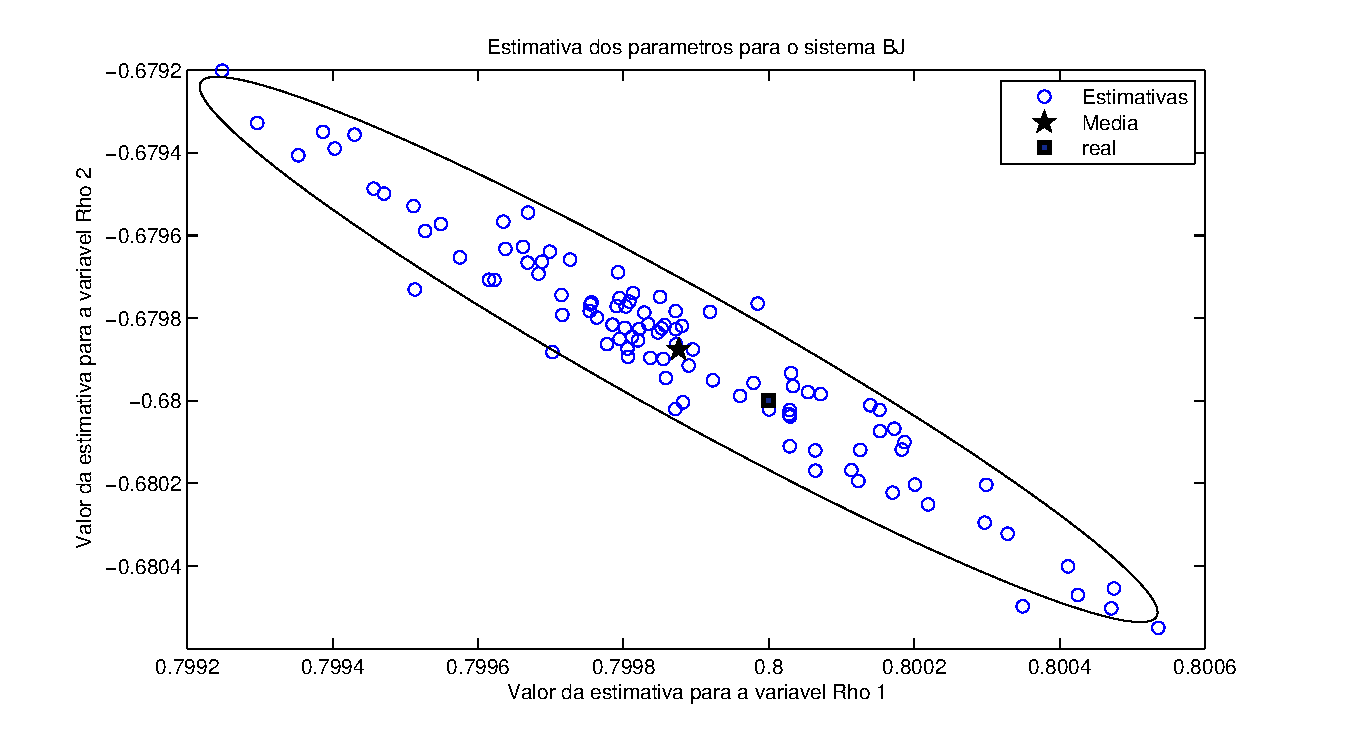
\includegraphics[width=0.95\columnwidth]{figures/vrft_bj_M10_var005.eps}
	\caption{100 estimativas Monte Carlo dos parametros $\rho_1$ e $\rho_2$ para o
	controlador apresentado em \eqref{eq:vrft_methos_ex_bj_c}}
	\label{fig:vrft_bj_M10_var005}
\end{figure}

Os parametros reais esperados para o controlador (equa��o \eqref{eq:vrft_methos_ex_bj_cd}) e a m�dia de todas
as estimativas (valor representado por uma estrela na Figura (\ref{fig:vrft_bj_M10_var005})) n�o s�o os
mesmos. Em uma situa��o onde o erro de polariza��o das estimativas n�o existe, o aumento de N (n�mero de
amostras) implica que esta diferen�a diminui, tendendo a zero. Em um cen�rio onde h� erro de polariza��o, se 
aumentarmos a vari�ncia do ruido do sistema, ser� observado um aumento desta diferen�a.

Na figura (\ref{fig:vrft_bj_M10_var02}) quadruplicou-se a vari�ncia do ruido inserido no sistema ($\sigma
_\upsilon ^2=0.02$). Observa-se ent�o que o erro de polariza��o existe na estimativa. Como descrito em
\cite{campi_leccini_savaresi2002} quando o m�todo do VRFT � utilizado com ruido nas amostras, a estimativa �
inevitavelmente polarizada. Neste mesmo trabalho � sugerido a utiliza��o de {\it{variaveis instrumentais}}
(Se��o (\ref{sec:si_par_estim_iv})) para que este erro de polariza��o seja minimizado.

\begin{figure}[htbp] 
	\center 
	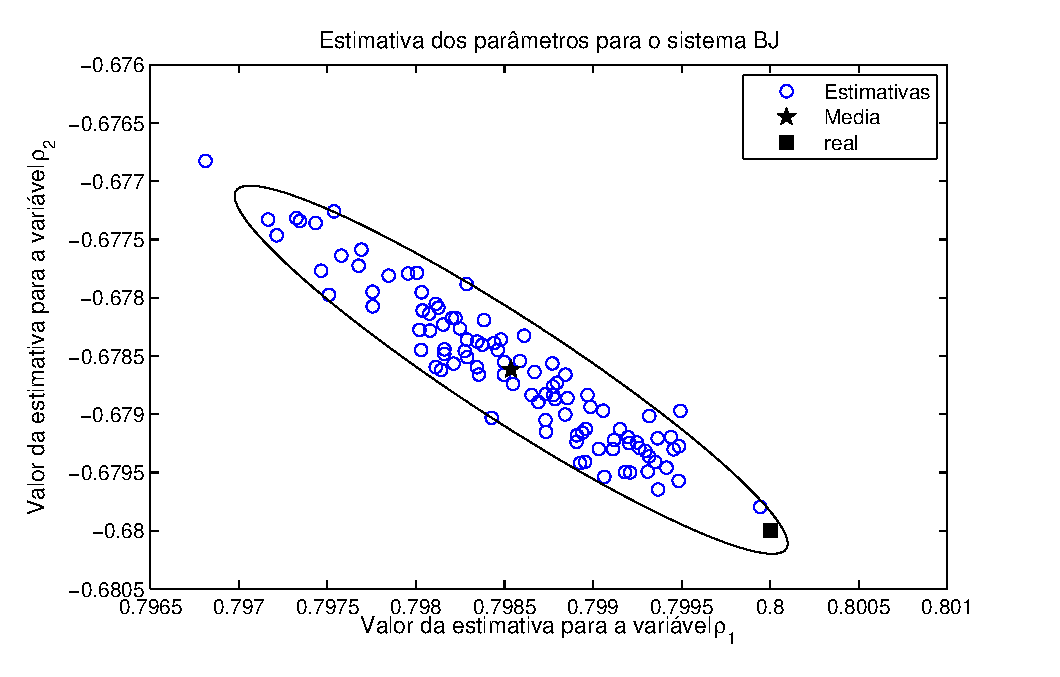
\includegraphics[width=0.95\columnwidth]{figures/vrft_bj_M10_var02.eps}
	\caption{100 estimativas Monte Carlo dos parametros $\rho_1$ e $\rho_2$ para o controlador apresentado em
	\eqref{eq:vrft_methos_ex_bj_c} com varancia do ruido de 0.02}
	\label{fig:vrft_bj_M10_var02}
\end{figure}

Utilizando o procedimento descrito na se��o (\ref{sec:vrft_framework_noise}) para dados corrompidos por ruido
o resultado obtido, para a mesma vari�ncia de $\sigma_\upsilon ^2=0.02$ do ruido, � apresentado na Figura
(\ref{fig:vrft_bj_M10_var02}).

\begin{figure}[htbp]
	\center
	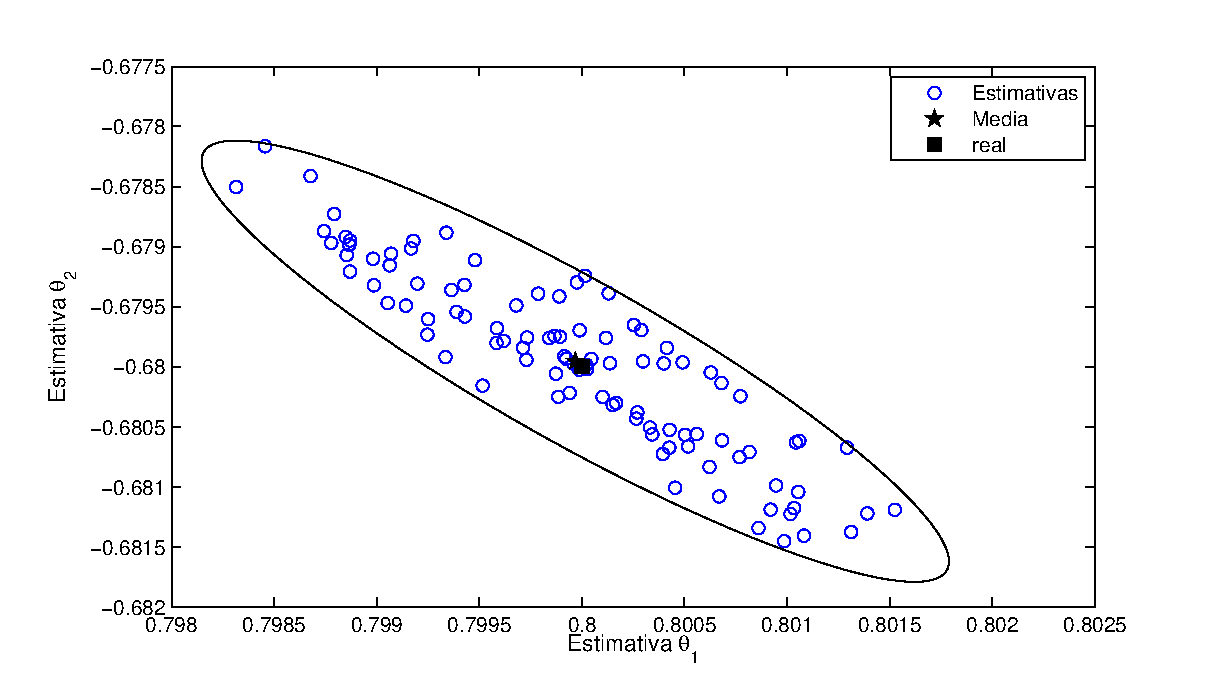
\includegraphics[width=0.95\columnwidth]{figures/vrft_bj_M10_var02_iv.eps}
	\caption{100 estimativas Monte Carlo dos parametros $\rho_1$ e $\rho_2$ para o
	controlador apresentado em \eqref{eq:vrft_methos_ex_bj_c} com varancia do
	ruido de 0.02. Utilizando vari�veis instrumentais para estimar os parametros.}
	\label{fig:vrft_bj_M10_var02_iv}
\end{figure}

Observa-se que o erro de polariza��o foi minimizado e que o resultado obtido possui um custo $J_{VR}^N(\theta)
= 5.1242$ e a vari�ncia dos parametros estimados foi de $0.5064e-06$ para $\rho_1$ e de $0.5495e-06$ para
$\rho_2$.

A fim de comparar o metodo VRFT utilizando e n�o utilizando variaveis instrumentais s�o apresentados abaixo as
Tabelas (\ref{table:vrft_method_bj}) e (\ref{table:vrft_method_bj_iv}) onde o custo $J_{MR}$ (equa��o
\eqref{eq:vrft_method_cost_func}) e o custo $J_{VR}^N$ (equa��o \eqref{eq:vrft_method_filter_criter_assim})
s�o apresentados para diferentes valores de vari�ncia do ruido para o mesmo sismtema BJ.

\begin{table*}[htbp]
\begin{center}
\caption{Valor dos custos $J_{VR}^N$ e $J_{MR}$ al�m da  vari�ncia das
estimativas para diferentes valores de $\sigma _\upsilon ^2$ quando o metodo
VRFT n�o utiliza vari�veis instrumentais para a estimativa dos parametros
$\rho$}
\label{table:vrft_method_bj}
\begin{tabular}{cccc}
\hline
        Vari�ncia $\sigma _\upsilon ^2$ & $J_{VR}^N(\theta)$ &
        $J_{MR}(\theta)$ & Vari�ncia estimativas $\rho$   \\
\hline
	    0.06    & 1.7893e-2 & 8.2367e-3 & 1.0e-05\;[0.4754    0.4434] \\
	    0.05    & 1.2515e-2 & 5.5366e-3 & 1.0e-05\;[0.2671    0.3244] \\
        0.04    & 8.1897e-3 & 3.6071e-3 & 1.0e-05\;[0.1534    0.1583] \\
        0.01    & 4.9665e-4 & 2.4402e-4 & 1.0e-06\;[0.0963    0.1035] \\
        0.005   & 1.2515e-4 & 5.6013e-5 & 1.0e-07\;[0.2999    0.3114] \\
        0.001   & 5.0036e-6 & 3.5734e-6 & 1.0e-08\;[0.1301    0.1223] \\
\hline
\end{tabular}
\end{center}
\end{table*} 
   

\begin{table*}[htbp]
\begin{center}
\caption{Valor dos custos $J_{VR}^N$ e $J_{MR}$ al�m da  vari�ncia das
estimativas para diferentes valores de $\sigma _\upsilon ^2$ quando o metodo
VRFT utiliza vari�veis instrumentais para a estimativa dos parametros $\rho$}
\label{table:vrft_method_bj_iv}
\begin{tabular}{cccc}
\hline
        Vari�ncia $\sigma _\upsilon ^2$ & $J_{VR}^N(\theta)$ &
        $J_{MR}(\theta)$ & Vari�ncia estimativas $\rho$   \\
\hline
	    0.06    & 45.1719  &  9.7345e-05 & 1.0e-05\;[0.5161    0.5332] \\
	    0.05    & 33.2600  &  2.0457e-05 & 1.0e-05\;[0.2481    0.2652] \\
        0.04    & 21.2652  &  1.1665e-04 & 1.0e-05\;[0.2040    0.2084] \\
        0.01    & 1.2956   &  8.9695e-06 & 1.0e-06\;[0.1246    0.1138] \\
        0.005   & 0.3264   &  7.4764e-06 & 1.0e-07\;[0.3063    0.2917] \\
        0.001   & 0.0126   &  5.2443e-07 & 1.0e-08\;[0.1059    0.1017] \\
\hline
\end{tabular}
\end{center}
\end{table*}

Utilizando vari�veis instrumentais observa-se que o custo $J_{MR}(\theta)$ � significativamente mais baixo
quando comparado com o metodo onde n�o s�o utilizadas vari�veis instrumentais. Demonstrando assim que o
comportamento desejado do sistema foi atingido com uma melhor aproxima��o.

%===============================================================================
\subsubsection{Controlador PID - sistema ARX}
\label{sec:vrft_examples_pid_arx}
%===============================================================================

Para um sistema {\it{ARX}} onde $G_0(z)$ e $H_0(z)$ podem ser definidos como:

\begin{equation}
G_{ 0 }(z)=\frac { z }{ (z-0.9)(z-0.8) } ,\quad \quad \quad H_{ 0 }(z)=\frac { z^2 }{ (z-0.9)(z-0.8) } 
\nonumber
\end{equation}

Deseja-se que o sistema em malha fechada comporte-se o mais pr�ximo poss�vel do modelo apresentado em
\eqref{eq:vrft_methos_ex_arx_M}.

\begin{equation}
M(z)=\frac { 0.4 }{ z-0.6 }
\label{eq:vrft_methos_ex_arx_M}
\end{equation}

Tem-se assim que o controlador ideal, aquele que ao ser inserido no sistema em
malha fechada apresentado na Figura (\ref{fig:vrft_db_control_loop}) propicia o
comportamento descrito por \eqref{eq:vrft_methos_ex_arx_M} �:

\begin{equation}
C_d(z)=\frac { 0.4(z - 0.9)(z-0.8) }{ z(z-1) }
\label{eq:vrft_methos_ex_arx_cd}
\end{equation}

Observa-se que este controlador pode ser representado como um controlador
{\it{PID}} como em \eqref{eq:vrft_methos_ex_arx_c}. 

\begin{equation}
C(z,\rho )=\frac { \rho _{ 1 }z^2+\rho _{ 2 }z+\rho _{ 3 } }{ z(z-1) } 
\label{eq:vrft_methos_ex_arx_c}
\end{equation}

Na Figura (\ref{fig:vrft_arx_M10_var005}) � apresentado o resultado da estimativa dos parametros do
controlador quando n�o s�o utilizados variaveis instrumentais. Obteve-se desta forma um custo
$J_{VR}^N(\theta) = 2.5008e-05$ e $J_{MR}(\theta) = 1.7746e-05$ al�m de uma vari�ncia para as estimativas de
$1.0e-07 \; [0.0364\;    0.1261\;    0.0377]$ para $\rho_1$, $\rho_2$ e $\rho_3$ respectivamente.

\begin{figure}[htbp] 
	\center 
	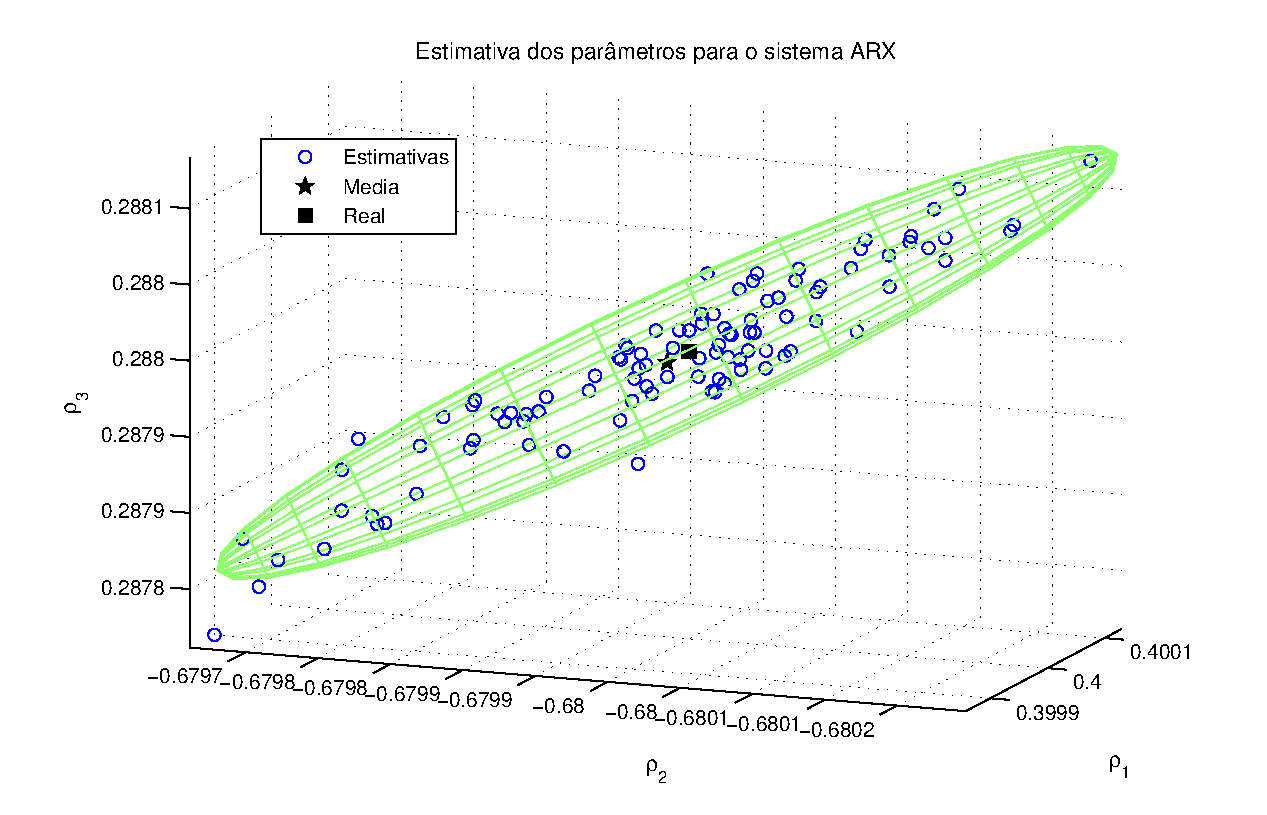
\includegraphics[width=0.95\columnwidth]{figures/vrft_arx_M10_var005_.eps}
	\caption{100 estimativas Monte Carlo dos parametros $\rho_1$, $\rho_2$ e $\rho_3$ para o controlador
	apresentado em \eqref{eq:vrft_methos_ex_arx_c} com varancia do ruido $\sigma_\upsilon ^2=0.005$}
	\label{fig:vrft_arx_M10_var005}
\end{figure}

Como j� foi observado a utiliza��o de variaveis instrumentais melhora significativamente o erro existente nas
estimativas. Desta forma as informa��es apresentadas a seguir ser�o feitas utilizando variaveis instrumentais.
Na figura (\ref{fig:vrft_arx_M10_var05_iv}) � apresentado a estimativa dos parametros do controlador para um
ruido com vari�ncia $\sigma_\upsilon ^2=0.05$. Observa-se que n�o h� erro de polariza��o nas estimativas. 
O custo para esta, e outas, estimativas � apresentado na Tabela (\ref{table:vrft_method_arx_iv}).

\begin{figure}[htbp] 
	\center 
	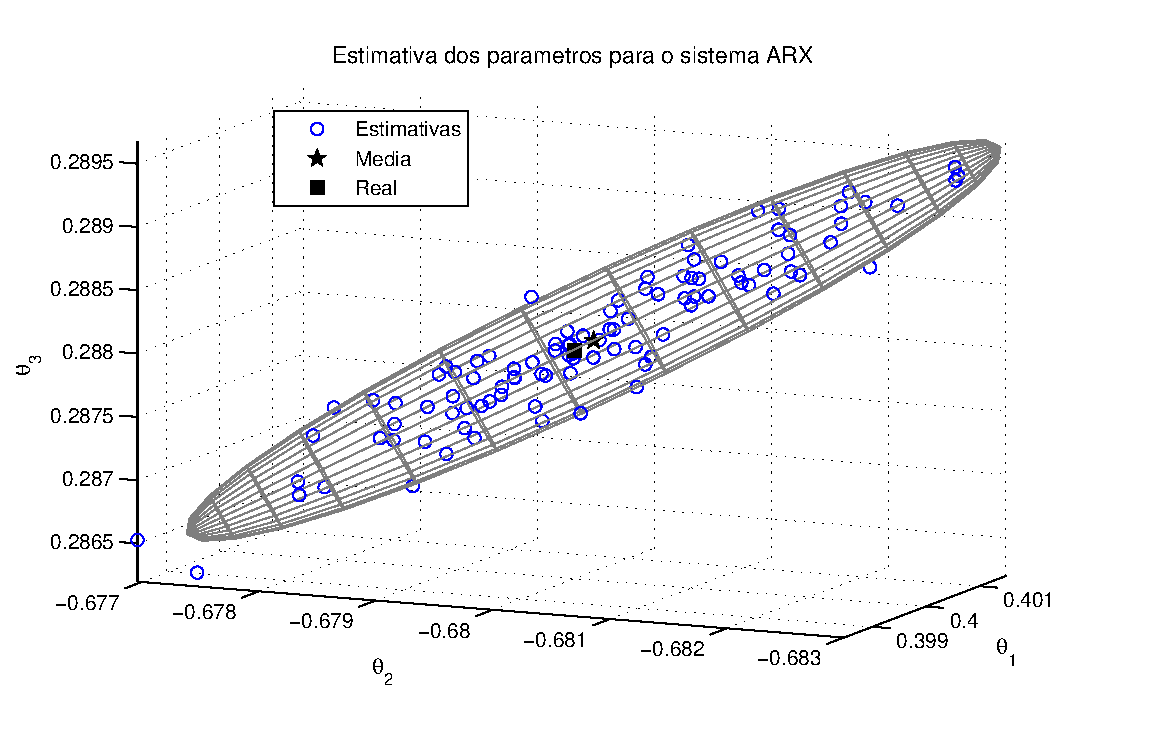
\includegraphics[width=0.95\columnwidth]{figures/vrft_arx_M10_var05_iv.eps}
	\caption{100 estimativas Monte Carlo dos parametros $\rho_1$, $\rho_2$ e $\rho_3$ para o controlador
	apresentado em \eqref{eq:vrft_methos_ex_arx_c} com varancia do ruido $\sigma_\upsilon ^2=0.05$ utilizando
	vari�veis instrumentais}
	\label{fig:vrft_arx_M10_var05_iv}
\end{figure}


\begin{table*}[htbp]
\begin{center}
\caption{Valor dos custos $J_{VR}^N$ e $J_{MR}$ al�m da  vari�ncia das
estimativas para diferentes valores de $\sigma _\upsilon ^2$ quando o metodo
VRFT utiliza vari�veis instrumentais para a estimativa dos parametros $\rho$ do controlador
\eqref{eq:vrft_methos_ex_arx_c}}
\label{table:vrft_method_arx_iv}
\begin{tabular}{cccc}
\hline
        Vari�ncia $\sigma _\upsilon ^2$ & $J_{VR}^N(\theta)$ &
        $J_{MR}(\theta)$ & Vari�ncia estimativas $\rho$   \\
\hline
	    0.1     & 10.0743e-3 & 2.2871e-3  & 1.0e-05\;[0.1253    0.4683    0.1600] \\
	    0.06    & 3.6093e-3  & 1.1279e-3  & 1.0e-05\;[0.0516    0.1793    0.0575] \\
	    0.05    & 2.5419e-3  & 1.2453e-3  & 1.0e-05\;[0.0344    0.1237    0.0416] \\
	    0.04    & 1.6013e-3  & 0.5106e-3  & 1.0e-06\;[0.2195    0.7908    0.2379] \\
        0.01    & 10.0077e-5 & 13.7142e-5 & 1.0e-07\;[0.1552    0.5469    0.1822] \\
        0.005   & 2.5081e-5  & 10.3482e-5 & 1.0e-07\;[0.0406    0.1260    0.0375] \\
		0.001   & 0.1009e-5  & 2.0487e-5  & 1.0e-09\;[0.1277    0.4035    0.1239]
\end{tabular}
\end{center}
\end{table*}

%===============================================================================
\subsubsection{Controlador n�o pertence a classe}
\label{sec:vrft_examples_not_in_class}
%===============================================================================


%===============================================================================
\subsection{VRFT em sistemas n�o lineares}
\label{sec:vrft_nonlinear}
%===============================================================================
ref: \cite{campi_savaresi2006}

\cite{lecchini_campi_savaresi_2dof}


\cite{Guardabassi}














































% ===============================================================================
\section{VRFT para sistemas n�o lineares}
\label{sec:vrft_nonlinear}
%===============================================================================

Como visto na se��o \ref{sec:vrft_vrft}, o m�todo VRFT tem um grande apelo, e produz resultados
significativamente satisf�torios para diversos modelos lineares. 

Nesta se��o o objetivo � demosntrar como este m�todo de coporta com sistemas n�o lineares. Duas
n�o linearidades ser�o apresentadas: est�ticas, para isso ser� utilizado o modelo de Wiener (apresentado na
se��o \ref{sec:nl_models_wiener_hammerstein}) e n�o linearidades din�micas, a classe de modelos escolhido
foram modelos NARMAX racionais (apresentados na se��o \ref{sec:nl_models_narmax_rat}).

A fun��o custo que pretende-se minimizar pode ser expressa como:

\begin{equation}
J(\theta)=\left \| y_{\theta}-M \tilde{r} \right \|^2
\label{eq:vrft_nl_j}
\end{equation} 

Onde $y_{\theta}=G\left [ C_{\theta}\left [ \tilde{r} -D y_{\theta} \right ] \right ]$ e $D$ � o atraso da
planta.

Desta forma o que se observa � que o custo a ser minimizado � dependente da planta que a-priori �
desconhecida. Ent�o � sugerido a minimiza��o de outra fun��o custo que possui a o mesmo minimo que
\eqref{eq:vrft_nl_j}: \cite{campi_savaresi2006}

\begin{equation}
J_{VRFT}(\theta)=\left \| F\left [ C_{\theta}[\tilde{e}] - F[\tilde{u}] \right ] \right \|^2
\label{eq:vrft_nl_jvrft}
\end{equation} 

Onde $F: \mathbb{R}^N\to \mathbb{R}^N$ � um filtro de que deve ser escolhido.

Em \cite{campi_savaresi2006} indica-se a utiliza��o do filtro:

\begin{equation}
F=(I-MD) \left ( \frac{\partial G\left [ u \right ]}{\partial u}|_{\tilde{u}} \right ) 
\label{eq:vrft_nl_filter}
\end{equation} 

Onde $ \frac{\partial G\left [ u \right ]}{\partial u}$ deve ser calculado a partir dos dados coletados.
Imprecis�es nesta estimativa apenas indicam que a segunda derivada de $J_{VRFT}$ n�o ir� precisamente
ter o mesmo m�nimo que $J$. \cite{campi_savaresi2006}

Devido ao custo e dificuldade de se obter $ \frac{\partial G\left [ u \right ]}{\partial u}$ e com o intuito
de utilizar o algotirmo de identifica��o de sistemas racionais apresentados na se��o
\ref{sec:nl_si_algorithms_rationals} optous-se em utilizar sistemas n�o lineares que pudessem ser aproximados
por equa��es n�o lineares racionais ou polinomiais. E desta forma utilizar a metodologia VRFT para gerar os
sinais $\bar{r}(t)$ e $e(t)$, e com isso alimentar o algoritmo de identifica��o de modelos racionais.

Como j� foi discutido, utilizando o m�todo VRFT, pode-se obter os sinais de alimenta��o do controlador, e de
posse do sinal de sa�da deste � poss�vel identificar o controlador que melhor atinge o almejado comportamento
da planta em malha fechada, descrito por $M(z)$.

Desta forma, o que foi alterado do m�todo classido do VRFT foi a utiliza��o do algoritmo de identifica��o de
modelos racionais, alimentando-o com o sinal de refer�ncia virtual $\bar{r}(t)$ e a sa�da $u(t)$.

A seguir ser�o apresentados alguns exemplos do uso deste procedimento e os resultados obtidos. Os exemplos
ser�o divididos em dois grupos principais: onde existe uma n�o linearidade est�tica na planta, e onde a n�o
linearidade � din�mica.

%===============================================================================
\subsection{N�o linearidades est�ticas}
\label{sec:vrft_nl_wiener}
%===============================================================================

Como n�o linearidade est�tica escolheu-se a classe de modelos de Wiener. Na Figura \ref{fig:vrft_nl_wiener} �
apresentado o diagrama de blocos do sistema, sendo $\Phi$ e $\Phi^{-1}$ os blocos n�o lineares da planta e do
controlador respectivamente.

\begin{figure}[htbp]
\center
\scalebox{1} % Change this value to rescale the drawing.
{
\begin{pspicture}(0,-0.92)(11.62,0.9)
\psline[linewidth=0.04cm,arrowsize=0.05291667cm 2.0,arrowlength=1.4,arrowinset=0.4]{->}(0.0,0.3)(0.8,0.3)
\pscircle[linewidth=0.04,dimen=outer](1.0,0.3){0.2}
\psline[linewidth=0.04cm,arrowsize=0.05291667cm 2.0,arrowlength=1.4,arrowinset=0.4]{->}(1.2,0.3)(2.0,0.3)
\psframe[linewidth=0.04,dimen=outer](3.2,0.7)(2.0,-0.1)
\psline[linewidth=0.04cm,arrowsize=0.05291667cm 2.0,arrowlength=1.4,arrowinset=0.4]{->}(3.2,0.3)(4.2,0.3)
\psframe[linewidth=0.04,dimen=outer](5.4,0.7)(4.2,-0.1)
\psframe[linewidth=0.04,dimen=outer](8.0,0.7)(6.8,-0.1)
\psline[linewidth=0.04cm,arrowsize=0.05291667cm 2.0,arrowlength=1.4,arrowinset=0.4]{->}(8.0,0.3)(9.0,0.3)
\psframe[linewidth=0.04,dimen=outer](10.2,0.7)(9.0,-0.1)
\psline[linewidth=0.04cm,arrowsize=0.05291667cm 2.0,arrowlength=1.4,arrowinset=0.4]{->}(5.4,0.3)(6.8,0.3)
\psline[linewidth=0.04cm,arrowsize=0.05291667cm 2.0,arrowlength=1.4,arrowinset=0.4]{->}(10.2,0.3)(11.6,0.3)
\psline[linewidth=0.04cm,arrowsize=0.05291667cm 2.0,arrowlength=1.4,arrowinset=0.4]{<-}(1.0,0.1)(1.0,-0.9)
\psline[linewidth=0.04cm](1.0,-0.9)(10.8,-0.9)
\psline[linewidth=0.04cm](10.8,-0.9)(10.8,0.3)
\usefont{T1}{ptm}{m}{n}
\rput(0.45828125,0.61){r(t)}
\usefont{T1}{ptm}{m}{n}
\rput(1.4946876,0.61){e(t)}
\usefont{T1}{ptm}{m}{n}
\rput(3.699375,0.61){v(t)}
\usefont{T1}{ptm}{m}{n}
\rput(6.089375,0.61){u(t)}
\usefont{T1}{ptm}{m}{n}
\rput(8.464531,0.61){$\omega(t)$}
\usefont{T1}{ptm}{m}{n}
\rput(10.899375,0.61){y(t)}
\psline[linewidth=0.04cm](1.2,0.1)(1.4,0.1)
\psframe[linewidth=0.04,linestyle=dashed,dash=0.16cm 0.16cm,dimen=outer](5.6,0.9)(1.8,-0.3)
\psframe[linewidth=0.04,linestyle=dashed,dash=0.16cm 0.16cm,dimen=outer](10.4,0.9)(6.6,-0.3)
\usefont{T1}{ptm}{m}{n}
\rput(3.5345314,-0.59){C(z)}
\usefont{T1}{ptm}{m}{n}
\rput(8.544531,-0.59){G(z)}
\usefont{T1}{ptm}{m}{n}
\rput(2.6745312,0.41){$\Phi^{-1}$}
\usefont{T1}{ptm}{m}{n}
\rput(9.524531,0.41){$\Phi$}
\usefont{T1}{ptm}{m}{n}
\rput(4.7745314,0.41){C'(z)}
\usefont{T1}{ptm}{m}{n}
\rput(7.384531,0.41){G'(z)}
\end{pspicture} 
}
\caption{Diagrama de blocos para um sistema n�o linear do tipo Wiener}
\label{fig:vrft_nl_wiener}
\end{figure}

Para este exmplo ser�o utilizadas as seguintes defini��es para o sistema:

\begin{equation}
G'(z)=\frac{0.5}{z-0.9}
\label{eq:vrft_nl_wiener_g}
\end{equation} 

\begin{equation}
M(z)=\frac{0.4}{z-0.6}
\label{eq:vrft_nl_wiener_m}
\end{equation}  

E a n�o linearidade escolhida foi:

\begin{equation}
\Phi(\omega)=y(k)=1.5\omega(k)+0.2\omega^3(k)
\label{eq:vrft_nl_wiener_phi}
\end{equation}  

Espera-se ent�o que por $M(z)$ ser linear, que o controlador tenha um bloco que seja o inverso de $\Phi$, para
que a n�o linearidade seja cancelada completamente.

Atingir uma express�o analitica que descreva $\Phi^{-1}$ n�o � uma tarefa simples. Optou-se ent�o por
aproximar esta fun��o por outro polin�mio de ordem 4:

\begin{equation}
\Phi^{-1}(e)= v(k) = a_1e(t) + a_2 e^2(k) +a_3 e^3(k) +a_4 e^4(k)
\label{eq:vrft_nl_wiener_phi_inv}
\end{equation}  

A partir da por��o linear da planta � poss�vel observar que a parte linear do controlador �timo ser�:

\begin{equation}
C_d(z)= \frac{0.8z-0.72}{z-1}
\label{eq:vrft_nl_wiener_cd}
\end{equation}  

Existe um integrador presente no controlador. Para evitar problemas de seguimento de refer�ncia optou-se por
n�o identificar esta parte do controlador. Mantendo o denominador como um integrador e identificando o
numerador, al�m do polin�mio da equa��o \eqref{eq:vrft_nl_wiener_phi_inv}.

Fazendo-se as substitui��es matem�ticas necess�rias, chega-se a express�o do sinal de sa�da do controlador que
se quer identificar:

\begin{equation}
u(k)=\begin{bmatrix}
\theta_1 & \theta_2 & \theta_3 & \theta_4 & \theta_5 & \theta_6 & \theta_7 & \theta_8
\end{bmatrix}
\begin{bmatrix}
e(k)\\ 
e^2(k)\\ 
e^3(k)\\ 
e^4(k)\\ 
e(k-1)\\ 
e^2(k-1)\\ 
e^3(k-1)\\ 
e^4(k-1)
\end{bmatrix}
\label{eq:vrft_nl_wiener_u}
\end{equation}  

Foram feitos 100 esperimentos de Monte Carlo e a m�dia das estimativas obtidas foi de:

\begin{equation}
\text{m�dia }\;\theta =\begin{bmatrix}
0.4471 \\ 0.0020 \\ -6.5105\times10^{-4} \\ -1.5959\times10^{-5} \\ -0.4043 \\ -0.0016 \\ 6.1194\times10^{-4}
\\ 1.4562\times10^{-5}
\end{bmatrix}^T
\nonumber
\end{equation}

Com um desvio padr�o de:

\begin{equation}
\text{m�dia }\;\theta = 1\times10^{-3}\begin{bmatrix}
0.2430 \\ 0.0246 \\ 0.0015 \\ 0.0001 \\ 0.2613 \\ 0.0259 \\ 0.0016 \\ 0.0001
\end{bmatrix}^T
\nonumber
\end{equation}

O custo $J_{MR}(\theta)= 0.3820$ (custo entre os sinais de sa�da do sistema obtido e esperado) e o custo
$J_{VR}=1.0119$ (custo dos sinais de sa�da do controlador, esperado e obtido).

Como a estimativa de $\Phi^{-1}$ � apenas uma aproxima��o do que esperaria-se ser a inversa de $\Phi$, a
classe de modelos escolhida para o controlador n�o consegue representar a totalidade do controlador ideal.

Na Figura \ref{fig:vrft_nl_wiener_step} � apresentado um comparativo entre o sinal de sa�da do sistema $M(z)$
quando submetido a um degrau unit�rio e o sinal do sistema com o controlador identificado.

\begin{figure}[htbp] 
	\center 
	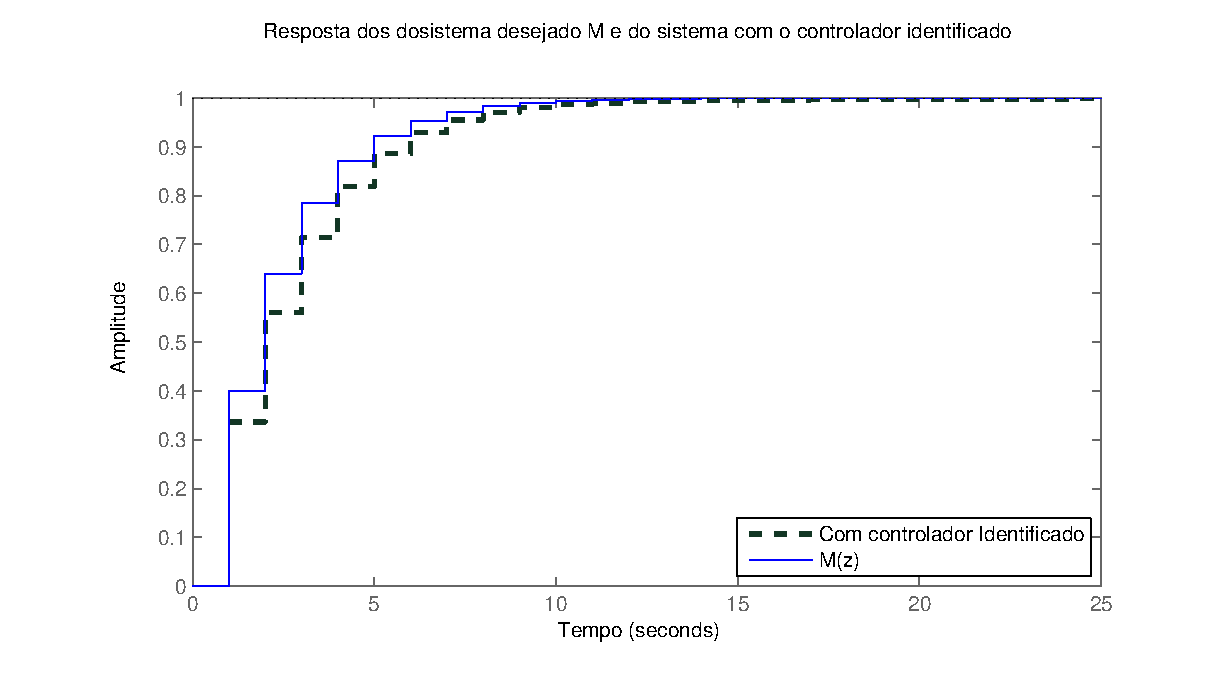
\includegraphics[width=0.95\columnwidth]{figures/vrft_nl_wiener_step.eps}
	\caption{resposta dos sistemas: desejado e obtido a um degrau unit�rio}
	\label{fig:vrft_nl_wiener_step}
\end{figure}

Na Figura \ref{fig:vrft_nl_wiener_vw_step} � apresentado o comportamento dos sinais de sa�da e entrada das n�o
linearidades $\Phi^{-1}$ e $\Phi$ respectivamente.

\begin{figure}[htbp] 
	\center 
	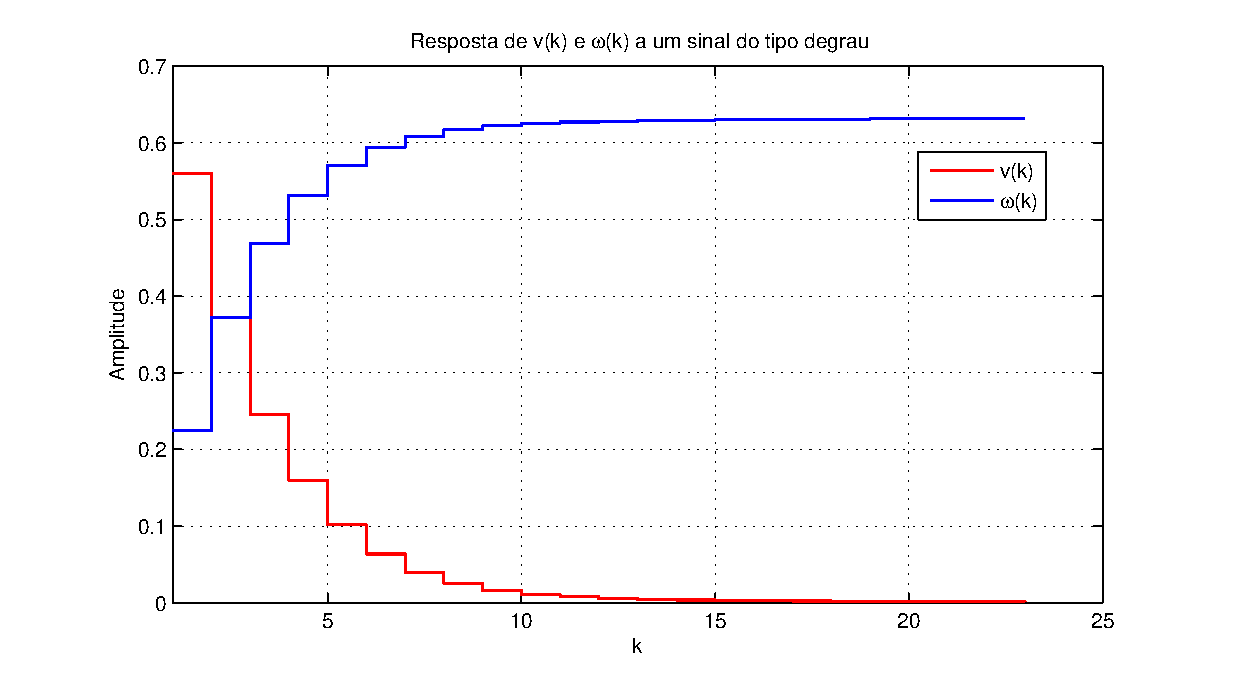
\includegraphics[width=0.95\columnwidth]{figures/vrft_nl_wiener_vw_step.eps}
	\caption{sinais $v(k)$ e $\omega(k)$ quando o sistema � alimentado por um degrau unit�rio}
	\label{fig:vrft_nl_wiener_vw_step}
\end{figure}

%===============================================================================
\subsection{N�o linearidades din�micas}
\label{sec:vrft_nl_dinamic}
%===============================================================================

ref: 

\cite{lecchini_campi_savaresi_2dof}


\cite{Guardabassi}














































%===============================================================================
\section{Considera��es Finais}
\label{sec:vrft_conclusions}
%===============================================================================


%===============================================================================

